\chapter{Études de cas et prototypes d’équipes IA autonomes} \label{chapitre:etudeCas}

\section{Cas d’étude : \textit{CodePori}}
\label{etudeCodePori}
\textit{CodePori}, proposé par \textcite{rasheed_codepori_2024}, vise à automatiser la génération de code pour des projets complexes à partir d’une description fonctionnelle en langage naturel.
Le système orchestre \textbf{six Agents IA} possédant chacun un rôle attitré bien défini, visible dans le tableau \ref{tab:mainTasks_MA} :

\begin{table}[H]
    \centering
    \begin{tabular}{|c|c|p{3cm}|p{7cm}|}
        \hline
        \textbf{No} & \textbf{Agent} & \textbf{Rôle principal} & \textbf{Contenu du Prompt} \\
        \hline
         1 & Manager & Segmentation des tâches & Prend la description du projet et segmente les tâches en modules plus petits et structurés \\
         \hline
         2 & Dev\_01 & Génération du code initial & Génère le code initial en se basant sur la description donnée \\
         \hline
         3 & Dev\_02 & Optimise le code généré & Affine et optimise le code généré par Dev\_01 \\
         \hline
         4 & Finalized\_01 & Assurance qualité du code & Joue un rôle d'assurance qualité et affine le code pour l'utilisation finale \\
         \hline
         5 & Finalized\_02 & Revue de qualité du code & Suggère un processus de révision itératif pour améliorer la qualité du code \\
         \hline
         6 & Verification & Vérification Finale du Code & Se concentre sur l'identification et la rectification des défauts de code que l'agent ci-dessus aurait pu manquer \\
         \hline
    \end{tabular}
    \caption{Tâche principales du Multi-agent, \parencite{rasheed_codepori_2024}}
    \label{tab:mainTasks_MA}
\end{table}

\textbf{Flux de travail.}
La figure \ref{fig:schemaCodePori} du papier illustre le pipeline : après avoir reçu la description du projet, le Manager décompose le projet, les Dev agents itèrent pour la génération du code, les Finalized font la revue croisée, puis le Verification\_Agent valide l’exécutable en cherchant les défauts que les Finalized auraient pu manquer. Toutes les requêtes sont acheminées par HTTPS vers l’API OpenAI, garantissant la traçabilité des échanges.

\begin{figure}[H]
    \centering
    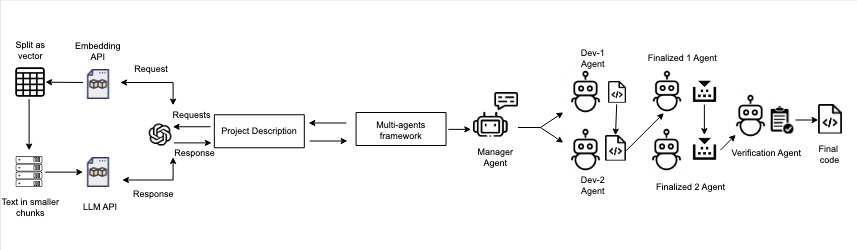
\includegraphics[width=1\linewidth]{images/CodePoriSchema.jpeg}
    \caption{Diagramme du workflow d'un système multi agent dirigé par IA pour la génération automatique de code \parencite{rasheed_codepori_2024}}
    \label{fig:schemaCodePori}
\end{figure}

\textbf{Évaluation.}
\begin{itemize}
  \item \textbf{Benchmark HumanEval} : 89\% de précision au test \textbf{Pass@1} (évaluant le taux de réussite au premier coup), surpassant plusieurs modèles de référence comme MetaGPT ou encore ChatDev.
  \item \textbf{Test manuel} sur 20 descriptions de projets : 85\% de code exécutable sans modifications (17 résultats concluants).
  \item \textbf{Coût et latence} : génération d’un projet complet "en quelques minutes" pour "quelques dollars"\footnote{Par exemple, pour un projet de détection de masque (visible sur la figure \ref{fig:projetsCodePori}) sur le visage, on a : 18 minutes pour 399 lignes de code et un coût de 1.02\$}. \cite{rasheed_codepori_2024}.
\end{itemize}

% rasheed_codepori_2024
% Our findings indicate that the proposed system is capable of generating accurate code for large and complex software projects within a few minutes.
% CodePori is able to generate running code for large-scale projects, aligned with the typical software development process within minutes, and at a cost of a few dollars.
%

\begin{figure}[H]
    \centering
    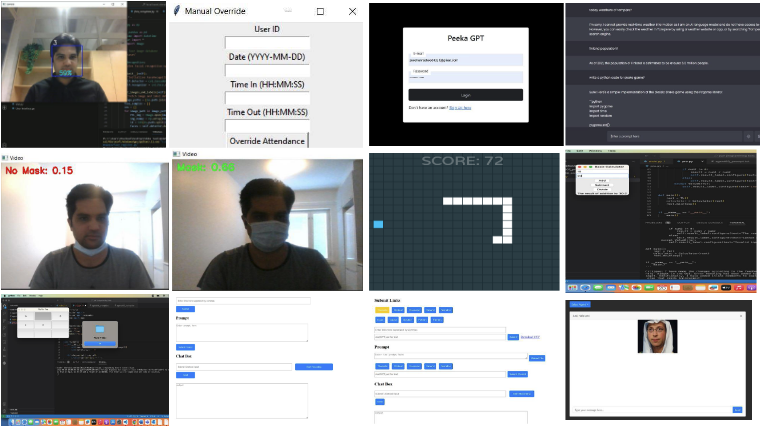
\includegraphics[width=0.75\linewidth]{images/CodePoriProjects.png}
    \caption{Logiciels développés par CodePori \parencite{rasheed_codepori_2024}}
    \label{fig:projetsCodePori}
\end{figure}

\paragraph{Forces et limites.}
CodePori démontre la faisabilité d’une équipe IA couvrant tout le cycle de développement (analyse → codage → tests → assurance qualité), mais l’étude souligne la dépendance à l’orchestration centrale et la nécessité d’itérations multiples pour obtenir un code pleinement fonctionnel.

\section{Cas d’étude : Agent-Driven Automatic Software Improvement}

\textcite{vallecillos_ruiz_agent-driven_2024} présente un projet doctoral qui vise à améliorer la maintenance logicielle en combinant \textbf{LLMs} et \textbf{agents IA} dans un cadre itératif de génération–révision.

\paragraph{Concept et architecture.}
La figure \ref{fig:schemaVallecillos} introduit un framework conceptuel composé d’un Agent LLM (Agent IA) et d’un critique (humain, outil ou autre LLM) échangeant sur des boucles continues pour affiner le code généré en donnant un retour entre chaque sortie (Output).  
\begin{figure}[H]
    \centering
    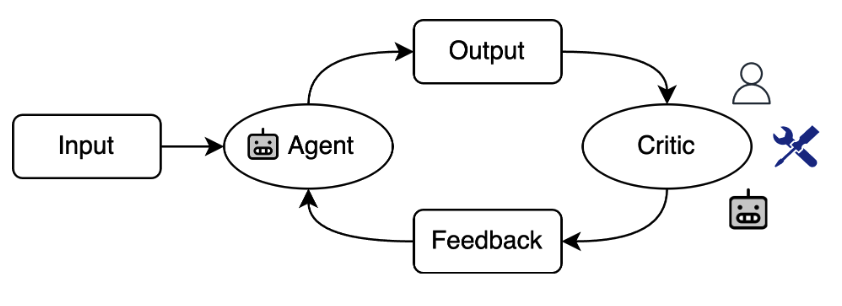
\includegraphics[width=0.75\linewidth]{images/VallecillosSchema.png}
    \caption{Framework conceptuel pour un Agent IA, \parencite{vallecillos_ruiz_agent-driven_2024}}
    \label{fig:schemaVallecillos}
\end{figure}

Trois scénarios d’interaction sont distingués (figure \ref{fig:schema2Vallecillos}) :  
\begin{enumerate}
  \item \textbf{Agent unique} agissant en autocontrôle;
  \item \textbf{Agents multiples} coopérant ou se spécialisant;
  \item \textbf{Human-in-the-loop} combinant expertise humaine et puissance de l’agent.
\end{enumerate}

\begin{figure}[H]
    \centering
    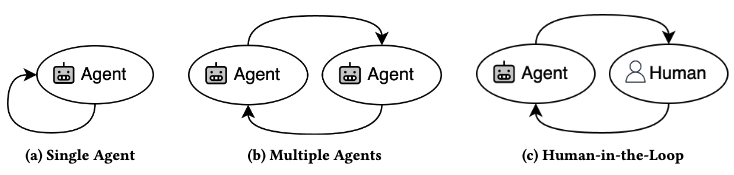
\includegraphics[width=0.75\linewidth]{images/VallecillosSchema2.png}
    \caption{Scenarios d’interactions entre Agents IA, \parencite{vallecillos_ruiz_agent-driven_2024}}
    \label{fig:schema2Vallecillos}
\end{figure}

\paragraph{Objectifs et contributions attendues.}
Le projet se déploie en trois phases correspondant aux questions de recherche :  
\begin{itemize}
  \item \textbf{RQ1} : comparer agent unique vs. usage one-shot d’un LLM sur des tâches d’amélioration de code;
  \item \textbf{RQ2} : étudier l’effet synergique d’équipes multi-agents spécialisées pour des scénarios complexes;
  \item \textbf{RQ3} : proposer de nouvelles méthodes de \emph{fine-tuning} tirant parti du processus itératif.
\end{itemize}

\paragraph{Boucles itératives et \emph{last-mile} problems.}
Les agents itératifs sont conçus pour résoudre les \textit{last-mile errors}, c’est-à-dire les bogues subtils apparaissant en toute fin de génération fonctionnelle. Chaque cycle d’itération permet :
\begin{enumerate}
  \item de recevoir un retour du critic ;
  \item de régénérer ou patcher la portion fautive ;
  \item d’améliorer progressivement sécurité, efficacité et style.
\end{enumerate}

\paragraph{Positionnement par rapport à l’état de l’art.}
L’auteur souligne que les approches mono-shot échouent souvent sur des codes complexes ou vulnérables, alors que des agents multi-itératifs sont plus compétents et plus aptes, par exemple, à régler un "last-mile problem".

\paragraph{Forces et limites.}
\begin{itemize}
  \item \textbf{Forces :} cadre générique, possibilité d’exploiter des experts spécialisés, amélioration continue via feedback loops.
  \item \textbf{Limites :} orchestration complexe, besoin d’une comparaison systématique des approches multi-agent, dépendance aux coûts d’appels API et à la qualité des critiques.
\end{itemize}

\section{Autres frameworks récents}

\subsection{Pipelines Auto-DevOps multi-agents}

\textcite{khan_ai-driven_2025} décrivent un cadre multi-agent intégré aux pratiques DevOps :  
des agents LLM distincts s’occupent de la planification de sprint, de la génération de code, de l’exécution automatique de tests et du déclenchement de pipelines CI/CD.  
Les auteurs rapportent une réduction du temps de développement et une meilleure cohérence entre le backlog et le code livré grâce à la distribution dynamique des tâches et au feedback continu entre agents.
% khan_ai-driven_2025
% Our study demonstrates that AI-driven automation can enhance various stages of the  software development lifecycle, including sprint planning, code generation, bug detection, and  testing. By leveraging specialized AI agents that collaborate dynamically, development teams can  streamline workflows, reduce errors, and accelerate project timelines.
%

\subsection{Retours d’expérience industriels ou open-source}

Dans un contexte industriel, \textcite{abbas_ai-driven_2024} montrent qu’une adoption progressive d’agents LLM pour la revue de code, la priorisation du backlog et l’automatisation des tests permet d’alléger la charge des développeurs et d’augmenter la productivité globale des équipes.  
Les agents interviennent notamment pour :
\begin{itemize}
  \item générer la documentation et détecter les risques en temps réel ;
  \item automatiser la revue de code et proposer des correctifs.
\end{itemize}

\section{Évaluation empirique}

La comparaison des prototypes et retours d'expérience fait ressortir trois indicateurs récurrents :

\begin{itemize}
  \item \textbf{Réduction du temps de développement} : les pipelines multi-agents permettent d’accélérer la planification et l’intégration continue \parencite{khan_ai-driven_2025}.
  \item \textbf{Amélioration de la productivité et de la détection d’erreurs} : l’automatisation des tâches répétitives (documentation, tests, revue) libère du temps pour les activités à forte valeur ajoutée \parencite{abbas_ai-driven_2024}.
  \item \textbf{Cohérence backlog $\leftrightarrow$ code livré} : la coordination d’agents spécialisés assure une meilleure traçabilité des exigences fonctionnelles jusqu’au code \parencite{khan_ai-driven_2025}.
\end{itemize}
